\documentclass[00-main.tex]{subfiles}
\begin{document}

\section*{Problem Two}

\subsection*{a.}
\begin{equation}
f_1(x_1, x_2) = x_1^2 + x_2^2 - 2; \: f_2(x_1, x_2) = x_1 - x_2
\end{equation}

\begin{equation}
f_1(1, 1) = 1^2 + 1^2 - 2 = 0; \: f_2(1, 1) = 1 - 1 = 0
\end{equation}

\begin{equation}
f_1(-1, -1) = (-1)^2 + (-1)^2 - 2 = 0; \: f_2(-1, -1) = (-1) - (-1) = 0
\end{equation}

This verifies that $\mathbf{f}(\mathbf{x}) = \mathbf{0}$ has two solutions: $x_1 = x_2 = 1$ and $x_1 = x_2 = -1$.

\begin{equation}
D\mathbf{f}(\mathbf{x})
=
\left[ 	
	\begin{array}{cc} 
		\frac{df_1}{dx_1} & \frac{df_1}{dx_2} \\ 
		\frac{df_2}{dx_1} & \frac{df_2}{dx_2}  
	\end{array} 
\right]
=
\left[ 	
	\begin{array}{cc} 
		2x_1 & 2x_2 \\ 
		1    & -1  
	\end{array} 
\right] 
\end{equation}

$D\mathbf{f}(\mathbf{x})$ is invertible iff $\mathbf{x}_1^{(0)} + \mathbf{x}_2^{(0)} \neq 0$.

\begin{equation}
[D\mathbf{f}(\mathbf{x})]^{-1}
=
\frac{1}{2(x_1+x_2)} 
\left[ 	
	\begin{array}{cc} 
		1 & 2x_2 \\ 
		1 & -2x_1  
	\end{array} 
\right] 
\end{equation}

Newton's method

\begin{equation}
\mathbf{f} (\mathbf{x}^{(0)} = D \mathbf{f} (\mathbf{x}^{(0)})(\mathbf{x}^{(1)} - \mathbf{x}^{(0)}) = \mathbf{0}
\end{equation}

\begin{equation}
\mathbf{x}^{(1)} = \mathbf{x}^{(0)} - \left[D\mathbf{f}(\mathbf{x}^{(0)})\right]^{-1} \mathbf{f} (\mathbf{x}^{(0)})
\end{equation}

\begin{equation}
\left[ 	
	\begin{array}{cc} 
		x_1^{(1)} \\ 
		x_2^{(1)}
	\end{array} 
\right] 
=
\left[ 	
	\begin{array}{cc} 
		x_1^{(0)} \\ 
		x_2^{(0)}  
	\end{array} 
\right] 
-
\frac{1}{2(x_1^{(0)} + x_2^{(0)})} 
\left[ 	
	\begin{array}{cc} 
		1 & 2x_2^{(0)} \\ 
		1 & -2x_1^{(0)}  
	\end{array} 
\right] 
\left[ 	
	\begin{array}{cc} 
		{x_1^{2}}^{(0)} + {x_2^2}^{(0)} - 2 \\ 
		x_1^{(0)} - x_2^{(0)}  
	\end{array} 
\right] 
\end{equation}

\begin{equation}
=
\left[ 	
	\begin{array}{cc} 
		x_1^{(0)} \\ 
		x_2^{(0)}  
	\end{array} 
\right] 
-
\frac{1}{2(x_1^{(0)} + x_2^{(0)})} 
\left[ 	
	\begin{array}{cc} 
		{x_1^{2}}^{(0)} + {x_2^2}^{(0)} + 2{x_2}^{(0)}(x_1^{(0)}-x_2^{(0)}) - 2 \\ 
		{x_1^{2}}^{(0)} + {x_2^2}^{(0)} 2{x_2^2}^{(0)}({x_2^2}^{(0)}-{x_2^2}^{(0)}) - 2 
	\end{array}
\right] 
\end{equation}

\begin{equation}
=
\left[ 	
	\begin{array}{cc} 
		2(x_1^{(0)} + x_2^{(0)})x_1^{(0)} - {x_1^{2}}^{(0)} + {x_2^2}^{(0)} + 2{x_2}^{(0)}(x_1^{(0)}-x_2^{(0)}) - 2 \\ 
		2(x_1^{(0)} + x_2^{(0)})x_2^{(0)} - {x_1^{2}}^{(0)} + {x_2^2}^{(0)} 2{x_2^2}^{(0)}({x_2^2}^{(0)}-{x_2^2}^{(0)}) - 2 
	\end{array}
\right] 
\end{equation}



\begin{minted}{matlab}
>> 
\end{minted}

\subsection*{b.}



\inputminted[linenos]{matlab}{newton_c.m}

\begin{figure}
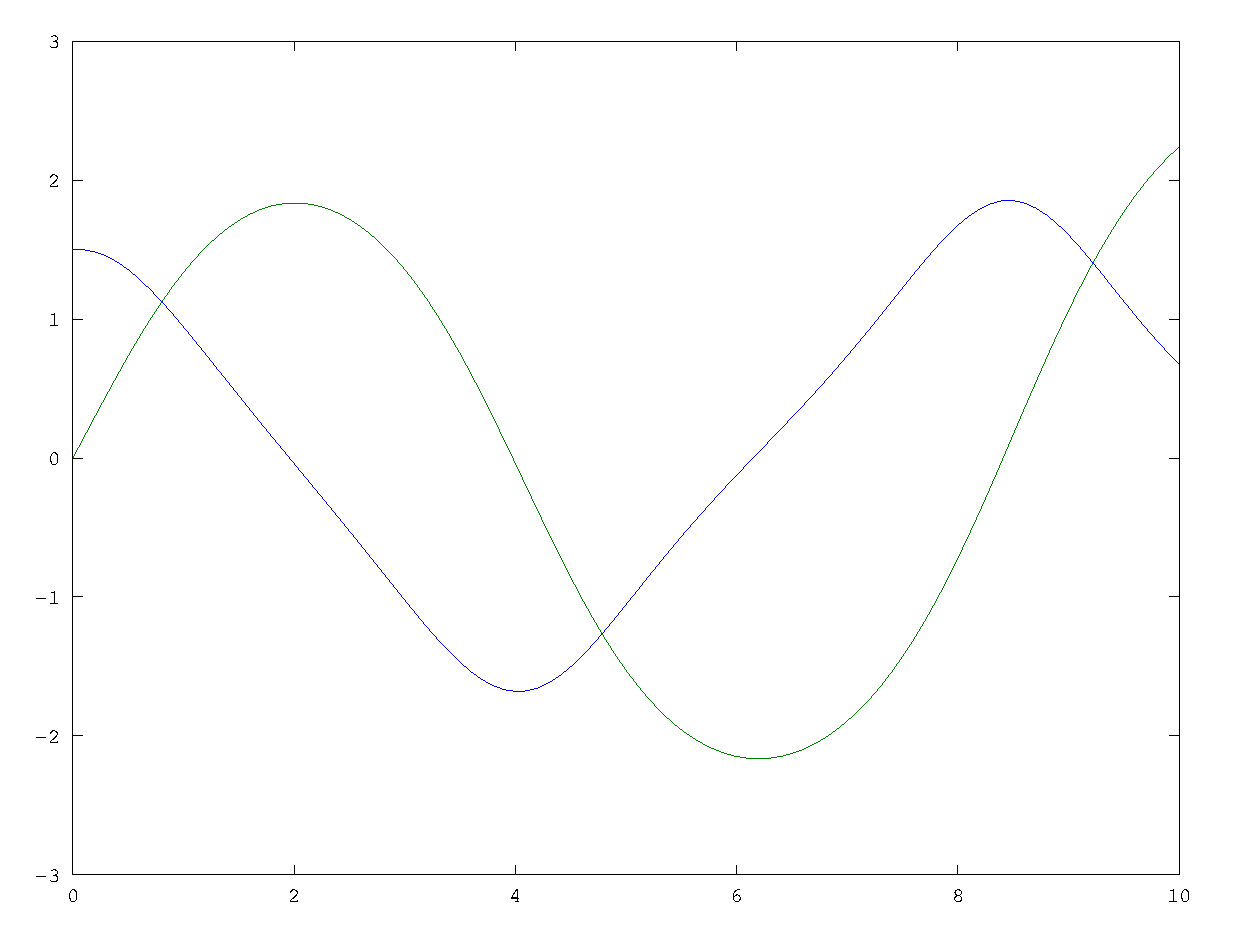
\includegraphics[width=\textwidth]{euler_plot}
\caption{Plot shows $y_1$ and $y_2$ that was found through Euler's method.}
\end{figure}


%\bibliosub
\end{document}